\documentclass[margin=5mm]{standalone}
\usepackage[dvipsnames]{xcolor}
\usepackage{pgfplots}
\usepackage{tikz}
\usepackage[tikz]{ocgx2}

\pgfplotsset{compat=1.18}
\begin{document}

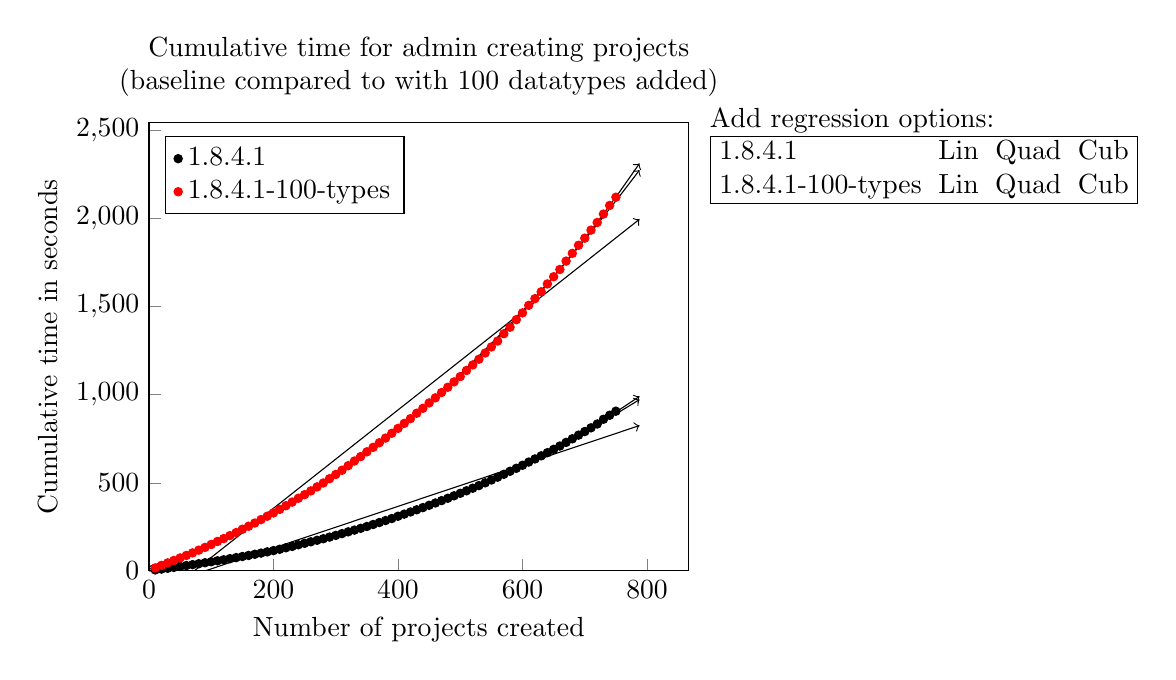
\begin{tikzpicture}
    \begin{axis}[
        align = center,
        legend pos = north west,
        legend cell align = left,
        xlabel = Number of projects created,
        ylabel = Cumulative time in seconds,
        xtick pos = left,
        ytick pos = left,
        scaled ticks = false,
        xmin = 0,
        ymin = 0,
        title = {Cumulative time for admin creating projects (baseline compared to with 100 datatypes added)},
        title style = {text width = 0.8\textwidth},
        legend entries={\switchocg{1.8.4.1}{1.8.4.1},\switchocg{1.8.4.1-100-types}{1.8.4.1-100-types}}]
        \begin{scope}[ocg = {ref = 1.8.4.1-Lin, status = invisible}]
            \plot[domain=0:788,->,forget plot] (\x,{-106.246609009008949442431912757456302642822265625 + 1.1813120938833570061632372016902081668376922607421875*(\x)^1});
        \end{scope}
        \begin{scope}[ocg = {ref = 1.8.4.1-Quad, status = invisible}]
            \plot[domain=0:788,->,forget plot] (\x,{13.8231942984079037017863811342976987361907958984375 + 0.245703236942445835122583730480982922017574310302734375*(\x)^1 + 0.00123106428544856780736560519784461575909517705440521240234375*(\x)^2});
        \end{scope}
        \begin{scope}[ocg = {ref = 1.8.4.1-Cub, status = invisible}]
            \plot[domain=0:788,->,forget plot] (\x,{1.197743756633374179187967456527985632419586181640625 + 0.4386907177074481634093672255403362214565277099609375*(\x)^1 + 0.00060042240024503934665844884221996835549362003803253173828125*(\x)^2 + 0.000000553194636143446168995477761620715995150021626614034175872802734375*(\x)^3});
        \end{scope}
        \begin{scope}[ocg = {ref = 1.8.4.1, status = visible}]
            \addplot[
                only marks,
                color = black,
                mark = *,
                mark size = 1.5 pt
            ]coordinates {(10,5.872)(20,10.636)(30,15.253)(40,20.237)(50,25.637)(60,30.421)(70,35.687)(80,40.994)(90,46.46)(100,52.207)(110,57.683)(120,63.3)(130,69.733)(140,75.653)(150,81.768)(160,87.895)(170,94.629)(180,101.239)(190,108.165)(200,115.264)(210,122.93)(220,131.43)(230,139.112)(240,148.517)(250,156.856)(260,165.397)(270,173.803)(280,182.721)(290,191.963)(300,201.59)(310,211.681)(320,221.708)(330,231.576)(340,241.683)(350,252.155)(360,263.396)(370,274.638)(380,285.76)(390,297.189)(400,310.327)(410,322.22)(420,334.346)(430,346.915)(440,359.336)(450,372.211)(460,385.38)(470,398.723)(480,412.219)(490,426.171)(500,440.311)(510,454.588)(520,469.143)(530,484.11)(540,499.631)(550,515.815)(560,531.803)(570,548.104)(580,565.421)(590,582.078)(600,599.308)(610,617.51)(620,635.103)(630,652.682)(640,670.739)(650,689.691)(660,708.49)(670,729.097)(680,749.432)(690,770.167)(700,790.534)(710,811.694)(720,833.47)(730,860.207)(740,883.029)(750,906.056)};
        \end{scope}
        \begin{scope}[ocg = {ref = 1.8.4.1-100-types-Lin, status = invisible}]
            \plot[domain=0:788,->,forget plot] (\x,{-202.407343783783431945266784168779850006103515625 + 2.788561431009956681492667485144920647144317626953125*(\x)^1});
        \end{scope}
        \begin{scope}[ocg = {ref = 1.8.4.1-100-types-Quad, status = invisible}]
            \plot[domain=0:788,->,forget plot] (\x,{24.794592906331207160519625176675617694854736328125 + 1.0181567295285429697315748853725381195545196533203125*(\x)^1 + 0.0023294798703702816744520731617740239016711711883544921875*(\x)^2});
        \end{scope}
        \begin{scope}[ocg = {ref = 1.8.4.1-100-types-Cub, status = invisible}]
            \plot[domain=0:788,->,forget plot] (\x,{-1.0139797564682890840259688047808595001697540283203125 + 1.4126560310666664843637363446759991347789764404296875*(\x)^1 + 0.0010403403767239439818570456708357596653513610363006591796875*(\x)^2 + 0.0000011308241172336298610285980348333367828672635369002819061279296875*(\x)^3});
        \end{scope}
        \begin{scope}[ocg = {ref = 1.8.4.1-100-types, status = visible}]
            \addplot[
                only marks,
                color = red,
                mark = *,
                mark size = 1.5 pt
            ]coordinates {(10,16.915)(20,31.527)(30,45.6)(40,59.481)(50,73.721)(60,87.923)(70,102.45)(80,117.964)(90,133.452)(100,150.364)(110,167.366)(120,183.542)(130,200.423)(140,217.679)(150,236.368)(160,253.562)(170,271.759)(180,291.233)(190,310.392)(200,329.356)(210,349.289)(220,369.947)(230,390.443)(240,412.299)(250,432.666)(260,453.877)(270,476.628)(280,498.769)(290,523.157)(300,547.095)(310,571.228)(320,597.012)(330,623.492)(340,648.594)(350,675.575)(360,700.989)(370,727.04)(380,753.554)(390,780.694)(400,808.449)(410,836.653)(420,863.853)(430,894.42)(440,922.538)(450,952.927)(460,981.74)(470,1011.95)(480,1041.681)(490,1072.218)(500,1102.331)(510,1137.084)(520,1168.408)(530,1200.833)(540,1235.891)(550,1270.51)(560,1303.851)(570,1345.388)(580,1382.428)(590,1424.831)(600,1463.743)(610,1506.339)(620,1544.264)(630,1583.212)(640,1627.742)(650,1668.552)(660,1709.79)(670,1757.26)(680,1801.286)(690,1846.928)(700,1887.384)(710,1933.025)(720,1976.137)(730,2024.009)(740,2072.868)(750,2119.502)};
        \end{scope}
    \end{axis}
    \begin{scope}
        \addtolength{\tabcolsep}{-0.3em}
        \node [below right, shape=rectangle, align=left](regressiontable) at (7,6) {
            Add regression options: \\
            \begin{tabular}{|llll|}
                \hline
                1.8.4.1 & \switchocg{1.8.4.1-Lin}{Lin} & \switchocg{1.8.4.1-Quad}{Quad} & \switchocg{1.8.4.1-Cub}{Cub} \\
                1.8.4.1-100-types & \switchocg{1.8.4.1-100-types-Lin}{Lin} & \switchocg{1.8.4.1-100-types-Quad}{Quad} & \switchocg{1.8.4.1-100-types-Cub}{Cub} \\
                \hline
            \end{tabular}
        };
    \end{scope}
\end{tikzpicture}

\end{document}